\section{Benchmark Design}
\label{sec:benchmark}

\begin{figure*}[t]
\centering
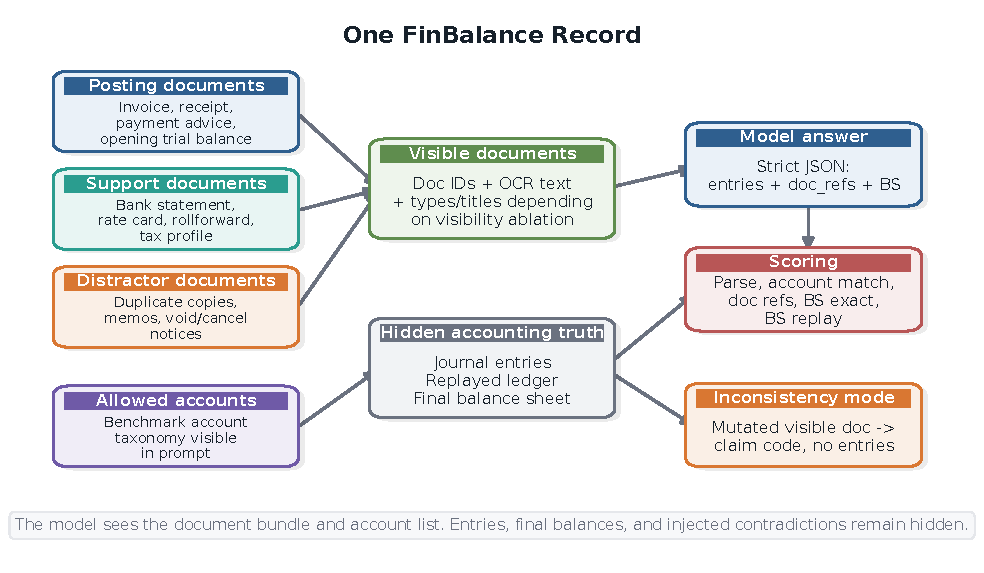
\includegraphics[width=0.96\textwidth]{figures/diag_dataset_packet.pdf}
\caption{One \benchmark{} record. The model sees a visible document bundle of posting, support, adjustment, and distractor documents plus the allowed account taxonomy. Hidden journal entries, balance sheets, and inconsistency labels remain available only to the deterministic scorer. For each visible document, the baseline prompt contains only its ID, type, title, and OCR text. The OCR-text-only condition retains only document IDs and OCR text, dropping type and title. Posting, support, and distractor annotations are used only by the generator and scorer and are never shown to the model.}
\label{fig:dataset-packet}
\end{figure*}

\paragraph{Task.}
A \benchmark{} record is a source-document bundle containing templated OCR text for one fiscal period of a synthetic business. Each bundle contains \emph{posting} documents (invoices, bills, statements, payment notices, and vouchers), \emph{support} documents (contracts, schedules, rate sheets, and certificates), \emph{adjustment} documents (period-end accruals, rollforwards, and reclassifications), an \emph{opening trial balance}, and neutralised but visually plausible \emph{distractor} documents. Given the bundle, opening trial balance, and allowed account list, the model returns JSON containing journal entries, a final balance sheet, and an inconsistency assessment. The journal entries comprise balanced debit and credit postings with an account, amount, date, and list of supporting-document references (\texttt{doc\_refs}). The balance sheet is structured by section, while the inconsistency assessment contains a flag, code, and justification.

\paragraph{Deterministic ledger ground truth.}
\benchmark{} fixes the chart of accounts, accounting policies, tax assumptions, and transaction generator, making its labels deterministic. The benchmark scores the canonical treatment defined by these visible policies. The human-authored specification defines the business scenarios, document schemas, tax and FX rules, lease, revenue, and deferred-tax treatments, supporting-document dependencies, distractors, and inconsistency perturbations. The generator selects scenarios, builds subledgers, renders PDF-style documents and OCR text, validates standard records, and replays the ledger to produce the journal entries and final balance sheet. \appfigref{fig:generation-inference} diagrams this generation and scoring workflow. \appfigrange{fig:dataset-samples}{fig:dataset-fx-clean} shows complete sample records. Every label is checked against double-entry invariants. No record is hand-labeled after generation.

\paragraph{Coverage.}
Records are stratified across eight industries (professional services, field services, retail, wholesale distribution, healthcare clinics, property management, manufacturing, and subscription SaaS), three period types (month, quarter, and year), and five difficulty levels (L1--L5). Difficulty is cumulative by construction. Each level retains the lower-level requirements while adding document volume, cross-document dependencies, jurisdictional complexity, temporal lookback, or advanced accounting concepts. \emph{Concept flags} include ASC~606 revenue recognition, lease accounting, deferred tax, asset disposals, FX scenarios, multi-jurisdictional tax with exemptions, and rollforwards. \appref{appx:dataset-details} gives the complete list. The main evaluation split contains $710$ records: four standard records for every industry--period--difficulty cell ($480$ total) and ten forced-inconsistency records for each of the 23 forced-inconsistency codes ($230$ total). We retain a compact $143$-record split for targeted ablations. The deterministic seeded generator allows users to generate new datasets, create held-out evaluation sets, and extend the scenario space without hand-labeling each record. \appref{appx:difficulty-validation} gives the construction rubric and practitioner judgments.

\paragraph{Forced-inconsistency records.}
A 23-code taxonomy of deliberate contradictions covers banking, billing, contract, jurisdictional, and reconciliation errors, including closing-balance conflicts, invoice-total mismatches, tax-total mismatches, and invalid exemption certificates. These records test whether a model recognizes that the source documents are internally inconsistent and withholds a fabricated balance sheet. In a forced-inconsistency record, the generator first builds a standard record and then applies a code-specific perturbation that makes the document bundle unreconcilable. The model must report that the bundle is inconsistent, emit the correct code, and leave the journal entries and balance sheet empty. Forced-inconsistency records are 32\% of the main evaluation split. \apptabref{tab:inconsistency-code-diagnostics} explains every code and reports per-code detection rates.

\paragraph{Metrics.}
For standard records, \bsexact{} measures whether the model's reported balance sheet matches ground truth to a tolerance of $0.01$. \bsrecon{} parses the model's journal entries, applies them to the opening balance with our deterministic ledger, and checks whether the resulting balance sheet matches ground truth. The difference $\bsrecon{}-\bsexact{}$ is the \aggGap{}. Because \bsrecon{} is an outcome-level replay metric, it can succeed even when the predicted entry set is not an exact posting-level match. Entry matching operates at the posting level. A strict match requires the debit account, credit account, rounded amount, and sorted supporting-document references to be correct. The lenient variant ignores supporting-document references. Balance-sheet and entry metrics do not apply to forced-inconsistency records because the correct output is an inconsistency flag and code with empty entries and an empty balance sheet. We therefore report \incCode{} separately as the rate of correct flag-plus-code predictions over the $230$ forced-inconsistency records. Strict end-to-end accuracy requires the reported balance sheet, journal entries, and supporting-document citations to match. Parse rate is reported over all records. \appref{appx:metrics-detail} gives the full matching procedure.

\paragraph{Ledger-feedback diagnostic.}
\label{sec:verifier}
One ablation uses the ledger as inference-time feedback to test whether a model can repair its reported balance sheet after receiving a deterministic consistency check. The evaluation procedure reads the model's structured answer, replays its entries, computes the implied balance sheet, and compares each account and section total with the model's reported balance sheet. It returns the full replayed balance sheet together with account-level and total deltas. For example:
\begin{quote}
\small\ttfamily
account: assets/Cash\\
submitted: \$48{,}500\\
replayed: \$51{,}300\\
delta: \$-2{,}800
\end{quote}
The feedback contains no ground-truth values or entry-correctness hints. The model receives one revision turn. This replay-and-revision protocol provides structured account-level feedback.
